%%%%%%%%%%%%%%%%%%%%%%%%%%%%%%%%%%%%%
%                                   %
% Compile with XeLaTeX and biber    %
%                                   %
% Questions or comments:            %
%                                   %
% joshua dot mcneill at uga dot edu %
%                                   %
%%%%%%%%%%%%%%%%%%%%%%%%%%%%%%%%%%%%%

\documentclass{beamer}
  % Read in standard preamble (cosmetic stuff)
  %%%%%%%%%%%%%%%%%%%%%%%%%%%%%%%%%%%%%%%%%%%%%%%%%%%%%%%%%%%%%%%%
% This is a standard preamble used in for all slide documents. %
% It basically contains cosmetic settings.                     %
%                                                              %
% Joshua McNeill                                               %
% joshua dot mcneill at uga dot edu                            %
%%%%%%%%%%%%%%%%%%%%%%%%%%%%%%%%%%%%%%%%%%%%%%%%%%%%%%%%%%%%%%%%

% Beamer settings
% \usetheme{Berkeley}
\usetheme{CambridgeUS}
% \usecolortheme{dove}
% \usecolortheme{rose}
\usecolortheme{seagull}
\usefonttheme{professionalfonts}
\usefonttheme{serif}
\setbeamertemplate{bibliography item}{}

% Packages and settings
\usepackage{fontspec}
  \setmainfont{Charis SIL}
\usepackage{hyperref}
  \hypersetup{colorlinks=true,
              allcolors=blue}
\usepackage{graphicx}
  \graphicspath{{../../figures/}}
\usepackage[normalem]{ulem}
\usepackage{enumerate}

% Document information
\author{M. McNeill}
\title[FREN2001]{Français 2001}
\institute{\url{joshua.mcneill@uga.edu}}
\date{}

%% Custom commands
% Lexical items
\newcommand{\lexi}[1]{\textit{#1}}
% Gloss
\newcommand{\gloss}[1]{`#1'}
\newcommand{\tinygloss}[1]{{\tiny`#1'}}
% Orthographic representations
\newcommand{\orth}[1]{$\langle$#1$\rangle$}
% Utterances (pragmatics)
\newcommand{\uttr}[1]{`#1'}
% Sentences (pragmatics)
\newcommand{\sent}[1]{\textit{#1}}
% Base dir for definitions
\newcommand{\defs}{../definitions}


  % Packages and settings
  \usepackage[backend=biber, style=apa]{biblatex}
    \addbibresource{../references/References.bib}

  % Document information
  \subtitle[Conversation Rules]{The Rules of Conversation}

  %% Custom commands
  % Subsection/frame titles
  \newcommand{\suboneone}{The cooperative principle}
  \newcommand{\subonetwo}{The maxims}
  \newcommand{\subonethree}{Flouting}
  \newcommand{\subonefour}{Practice}
  % Example conversation violating the maxim of relevance
  \newcommand{\relevance}{
    \begin{tabular}{r @{: } l}
      Kim   & \uttr{How are you today?} \\
      Sandy & \uttr{Oh, Harrisburg is the capital of Pennsylvania.} \\
      Kim   & \uttr{Really? I thought the weather would be warmer.} \\
      Sandy & \begin{tabular}[t]{@{} l @{}}
                `Well, in my opinion, the soup could use a little \\
                more salt.'
              \end{tabular}
    \end{tabular}
  }

\begin{document}
  % Read in the standard intro slides (title page and table of contents)
  %%%%%%%%%%%%%%%%%%%%%%%%%%%%%%%%%%%%%%%%%%%%%%%%%%%%%%%%%%%%%%%%
% This is a standard set of intro slides used in for all slide %
% documents. It basically contains the title page and table of %
% contents.                                                    %
%                                                              %
% Joshua McNeill                                               %
% joshua dot mcneill at uga dot edu                            %
%%%%%%%%%%%%%%%%%%%%%%%%%%%%%%%%%%%%%%%%%%%%%%%%%%%%%%%%%%%%%%%%

\begin{frame}
  \titlepage
  \tiny{Office: % Basically a variable for office hours location
Gilbert 121\\
        Office hours: % Basically a variable for office hours
 lundi, mercredi, vendredi 10:10--11:10
}
\end{frame}

\begin{frame}
  \tableofcontents[hideallsubsections]
\end{frame}

\AtBeginSection[]{
  \begin{frame}
    \tableofcontents[currentsection,
                     hideallsubsections]
  \end{frame}
}


  \section{The Rules of Conversation}
    \subsection{\suboneone}
      \begin{frame}{\suboneone}
        \begin{center}
          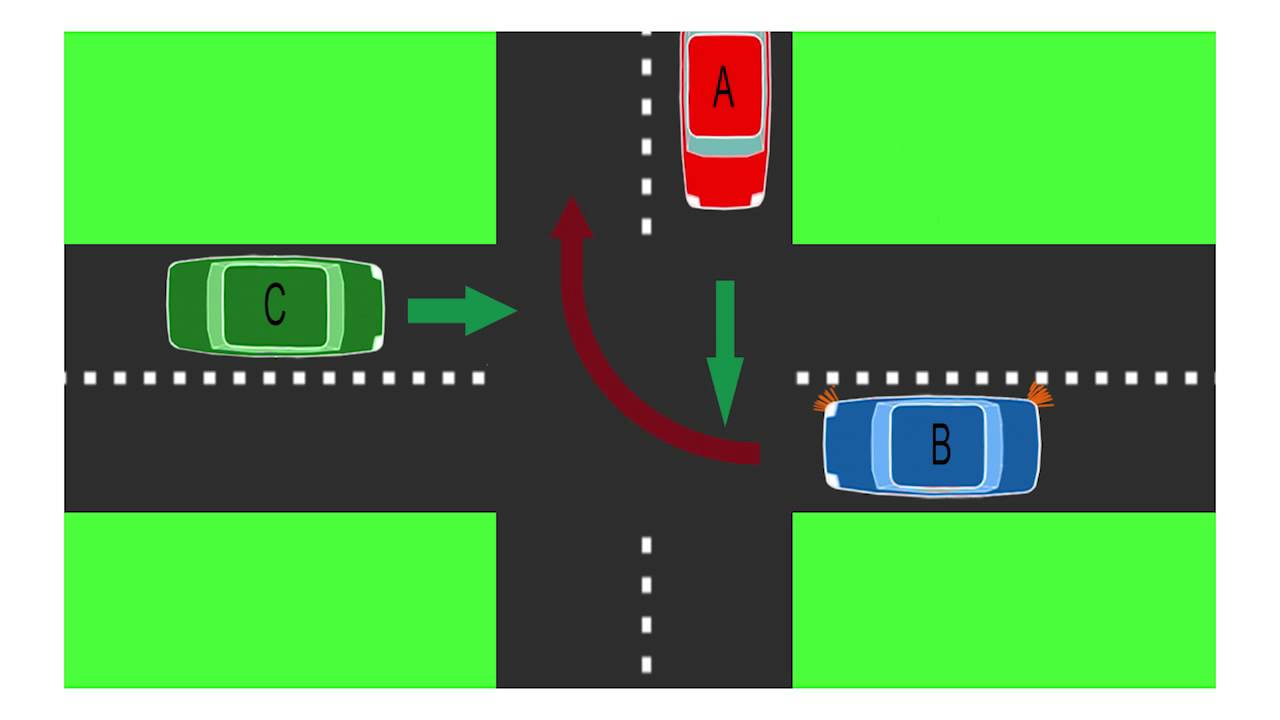
\includegraphics[scale=0.18]{stop.jpg}
        \end{center}
        \begin{block}{Who has the right of way?}
          \uncover<2->{
            $A \rightarrow B \rightarrow C$
            \begin{itemize}
              \item<3-> What happens if $B$ goes first?
            \end{itemize}
          }
        \end{block}
      \end{frame}

      \begin{frame}{\suboneone}
        \begin{alertblock}{Cooperative principle \parencite{grice_logic_1989}}
          % Cooperative principle
The set of assumptions that speakers work under when conversing

        \end{alertblock}
        \begin{block}<2->{Why doesn't this conversation work?}
          \relevance
        \end{block}
      \end{frame}

    \subsection{\subonetwo}
      \begin{frame}{\subonetwo}
        \begin{block}{The four maxims of the cooperative principle}
          \begin{itemize}
            \item The maxim of relevance
            \item The maxim of quality
            \item The maxim of quantity
            \item The maxim of manner
          \end{itemize}
        \end{block}
      \end{frame}

      \begin{frame}[t]{\subonetwo}
        \begin{alertblock}{The maxim of relevance}
          % Maxim of relevance
The idea that a speaker should only say things that are pertinent to the conversation

        \end{alertblock}
        \only<2>{
          \begin{block}{This example violated this maxim repeatedly}
            \relevance
          \end{block}
        }
        \only<3-5>{
          \begin{example}
            \begin{tabular}{r @{: } l}
              Alana & \uttr{Is Jamie dating anyone these days?} \\
              Sam   & \uttr{Well, she goes to Atlanta every weekend.}
            \end{tabular}
          \end{example}
          \only<3-4>{
            \begin{block}{What does Sam mean, and how do you know?}
              \uncover<4->{
              Jamie is dating someone in Atlanta, because we assume that Sam is being relevant and so infer the indirect meaning
              }
            \end{block}
          }
          \only<5->{
            \begin{alertblock}{Implicature}
              % Implicature
That information which is indirectly communicated through an utterance, understood using the cooperative principle maxims

            \end{alertblock}
          }
        }
        \only<6>{
          \begin{alertblock}{}
            The maxim of relevance doesn't prevent topics from being changed
          \end{alertblock}
          \begin{example}
            \begin{tabular}{r @{: } l}
              Rachel  & \begin{tabular}[t]{@{} l @{}}
                          `We should think of something fun to do this \\
                          weekend.'
                        \end{tabular} \\
              Sarah   & \uttr{Can we talk about something from class instead?}
            \end{tabular}
            \begin{itemize}
              \item \lexi{Instead} indicates an attempt to change what's relevant
            \end{itemize}
          \end{example}
        }
      \end{frame}

      \begin{frame}[t]{\subonetwo}
        \begin{alertblock}{The maxim of quality}
          % Maxim of quality
The idea that a speaker should only say what they believe to be true and have evidence for

        \end{alertblock}
        \begin{block}<2->{What counts as evidence varies according to context}
          \uttr{A purple toothed spider's venom won't kill you,} uttered:
          \begin{enumerate}
            \item by a biologist at a science conference
            \item by your friend who was once bitten by one
          \end{enumerate}
        \end{block}
        \begin{block}<2->{Do these violate the maxim?}
          \uncover<3->{
            Neither does, even though their evidence is different
          }
        \end{block}
      \end{frame}

      \begin{frame}[t]{\subonetwo}
        \begin{alertblock}{The maxim of quantity}
          % Maxim of quantity
The idea that a speaker should not more and no less information than is necessary

        \end{alertblock}
        \only<2>{
          \begin{example}
            Responding to \uttr{Why are you late?} with:
            \begin{enumerate}
              \item \uttr{Because.}
              \item \uttr{I wanted to go get a sandwich, but I wanted black olives and the first place was out of them, so I went to the other, but my friend called me on the way and \ldots}
            \end{enumerate}
          \end{example}
          \begin{block}{}
            These both violate the maxim
          \end{block}
        }
        \only<3-4>{
          \begin{block}{Implicature returns}
            \begin{tabular}{r @{: } l}
              Gail  & \uttr{Can you run a marathan without stopping?} \\
              Kim   & \uttr{I can run ten miles.}
            \end{tabular}
          \end{block}
          \begin{block}{Can Kim run a marathon?}
            \uncover<4->{
              No, only ten miles, unless she's violating the maxim
            }
          \end{block}
        }
      \end{frame}

      \begin{frame}[t]{\subonetwo}
        \begin{alertblock}{The maxim of manner}
          % Maxim of manner
The idea that a speaker should communicate using clear and unambiguous language

        \end{alertblock}
        \only<2>{
          \begin{alertblock}{}
            Unlike the other maxims, this one has nothing to do with the information communicated
          \end{alertblock}
        }
        \only<3-4>{
          \begin{example}
            \begin{enumerate}
              \item \#\uttr{Covert prestige explains his informal idiolect.}
              \item \#\uttr{He promised to call at noon.}
            \end{enumerate}
          \end{example}
          \begin{block}{}
            \begin{itemize}
              \item What does (1) mean?
              \item<4-> In (2), did he promise at noon or will he call at noon?
            \end{itemize}
          \end{block}
        }
      \end{frame}

    \subsection{\subonethree}
      \begin{frame}[t]{\subonethree}
        \begin{alertblock}{Flouting a maxim}
          % Flouting a maxim
When a maxim of the cooperative principle is purposefully not followed in a way that's obvious to the listener

        \end{alertblock}
        \only<2>{
          \begin{example}
            Someone who hasn't taken linguistics to you:
            \begin{tabular}{r @{: } l}
              Them  & \uttr{You're not so smart.} \\
              You   & \#\uttr{I know which diphthong you used in \lexi{so}.}
            \end{tabular}
          \end{example}
          \begin{block}{}
            This is flouting of the maxim of manner
          \end{block}
        }
        \only<3-4>{
          \begin{example}
            Someone makes an unbelievable claim:
            \begin{tabular}{r @{: } l}
              You & \#\uttr{And I'm the Queen of England!}
            \end{tabular}
          \end{example}
          \begin{block}{Which maxim is this flouting?}
          \uncover<4->{
            The maxim of quality
          }
          \end{block}
        }
        \only<5-6>{
          \begin{example}
            Someone suddenly enters the room while you're discussing them, and you change the subject:
            \begin{tabular}{r @{: } l}
              You & \begin{tabular}[t]{l}
                      \#`So how about them Falcons? Definitely not as \\
                      good as the Saints.'
                    \end{tabular}
            \end{tabular}
          \end{example}
          \begin{block}{Which maxim is this flouting?}
            \uncover<6->{
              The maxim of relevance
            }
          \end{block}
        }
        \only<7-8>{
          \begin{example}
            Your employer asks you to describe a bad co-worker's qualifications for a promotion:
            \begin{tabular}{r @{: } l}
              You & \#\uttr{They wear nice shoes.}
            \end{tabular}
          \end{example}
          \begin{block}{Which maxim is this flouting?}
            \uncover<8->{
              The maxim of quantity
            }
          \end{block}
        }
      \end{frame}

    \subsection{\subonefour}
      \begin{frame}{\subonefour}
        \begin{block}{Try these}
          \textcite{dawson_language_2016}, chapter 7 exercises 12 and 23
        \end{block}
      \end{frame}

      \begin{frame}{References}
        \printbibliography
      \end{frame}
\end{document}
